\documentclass[a4paper,11pt]{report}

\usepackage[polish]{babel}
\usepackage{packages/sleek}
\usepackage{packages/sleek-title}
\usepackage{packages/sleek-listings}

\institute{Instytut Chemii Bioorganicznej PAN}
\faculty{Analiza danych snRNA-seq}
\title{EBF2 jako marker do rozdziału jąder Purkinjego}
\subtitle{Dwa twierdzenia i ich weryfikacja}
\author{\textit{Analiza}\\Mikołaj \textsc{Rurad}}
\date{\today}

\begin{document}

\maketitle

\clearpage
\pagenumbering{roman}
\tableofcontents
\clearpage
\pagenumbering{arabic}

\chapter{Dane}

\section{Skąd pochodzą dane}

\paragraph{Atlas móżdżku myszy.}
Kozareva V. i wsp., \textit{A transcriptomic atlas of mouse cerebellar cortex
comprehensively defines cell types}, \textit{Nature} 2021; 598(7879): 214--219.
Numer akcesyjny GEO: \textbf{GSE165371}.

\begin{itemize}
    \item \url{https://www.ncbi.nlm.nih.gov/geo/query/acc.cgi?acc=GSE165371}
    \item DOI: \url{https://doi.org/10.1038/s41586-021-03220-z}
    \item Kod autorów: \url{https://github.com/MacoskoLab/cerebellum-atlas-analysis}
\end{itemize}

Metoda: snRNA-seq, 10x Chromium V3, jądra z kory móżdżku dorosłej myszy,
16 płacików. Macierz zawiera \textbf{24 409 genów} i \textbf{611 034 jąder}
po kontroli jakości. Komórek Purkinjego jest \textbf{16 634}, podzielonych przez
autorów na 9 podtypów: siedem oznaczonych jako Aldoc dodatnie (10 427 jąder)
i dwa jako Aldoc ujemne (6 207 jąder).

\paragraph{Białko EBF2.}
\begin{itemize}
    \item UniProt (mysz, \texttt{O08792}): \url{https://www.uniprot.org/uniprotkb/O08792/entry}
    \item Model przestrzenny AlphaFold: \url{https://alphafold.ebi.ac.uk/entry/O08792}
    \item Praca wiążąca EBF2 z zebriną (Chung i wsp. 2008): \url{https://pubmed.ncbi.nlm.nih.gov/18403128/}
\end{itemize}

\paragraph{Przeciwciała przeciw EBF2.}
\begin{itemize}
    \item R\&D Systems \texttt{AF7006}, owcze, reaktywność z myszą zadeklarowana:\\
          \url{https://www.rndsystems.com/products/human-mouse-ebf-2-antibody_af7006}
    \item Wersje sprzężone z barwnikiem: \texttt{AF7006P} (PE) oraz \texttt{AF7006J}
          (Janelia Fluor 646)
    \item Atlas Antibodies \texttt{HPA003954} i \texttt{HPA055101}:\\
          \url{https://www.proteinatlas.org/ENSG00000221818-EBF2/antibody}
\end{itemize}

\section{Kod}

Wszystkie liczby w tym dokumencie pochodzą z policzonych skryptów. Repozytorium:

\begin{center}
\url{https://github.com/mikolajrura/pc-zebrin-sorting}
\end{center}

Odnośniki do poszczególnych skryptów w dalszej części dokumentu wskazują pliki
w katalogu \texttt{scripts/} tego repozytorium. Repozytorium jest prywatne, więc
wymaga nadania dostępu.

\chapter{Twierdzenie pierwsze}

\section{Treść twierdzenia}

\begin{quote}
Komórki Purkinjego oznaczone przez Kozarevą jako Aldoc dodatnie i Aldoc ujemne
różnią się ilością mRNA genu \textit{Ebf2}. Grupa Aldoc ujemna ma go wyraźnie więcej.
\end{quote}

\section{Jak to policzyłem}

\paragraph{Krok 1, pobranie.}
Z GEO pobrano trzy pliki: macierz \texttt{cb\_adult\_mouse.mtx.gz} (3,1 GB),
listę 611 034 kodów kreskowych i listę 24 409 nazw genów. Z repozytorium autorów
pobrano tabelę metadanych z przypisaniem każdego jądra do typu komórki i podtypu.

\paragraph{Krok 2, przygotowanie.}
Skrypt \texttt{00\_prep\_map.py} łączy kody kreskowe z metadanymi. Jest tu pułapka,
którą trzeba było obejść: dwanaście próbek ma inną nazwę w GEO niż w metadanych
autorów, na przykład \texttt{VI2a\_F002} kontra \texttt{DECa\_F002}. Naiwne połączenie
gubi 1 167 komórek Purkinjego, czyli 7 procent, w tym trzy czwarte jąder z płacika
Culmen. Skrypt stosuje mapowanie nazw przed połączeniem.

Skrypt \texttt{01\_extract.sh} wycina z dużej macierzy tylko kolumny odpowiadające
komórkom Purkinjego, czytając plik strumieniowo. Cała macierz nie mieści się
w pamięci tej stacji roboczej.

Skrypt \texttt{02\_build\_h5ad.py} składa wynik w plik \texttt{purkinje\_cells\_v2.h5ad}
o wymiarach 16 634 na 24 409 i sprawdza go: dla 16 538 z 16 634 komórek liczba
niezerowych genów zgadza się z metadanymi co do jedności. Etykieta Aldoc dodatni
lub ujemny bierze się \textbf{wyłącznie z nazwy podtypu nadanej przez autorów pracy},
nie z żadnego progu ustawionego przeze mnie.

\paragraph{Krok 3, wynik.}
Zliczenia znormalizowano do 10 000 na jądro (jednostka CP10K) i porównano obie grupy.

\section{Wyniki}

\begin{table}[h]
\centering
\begin{tabular}{lrr}
\toprule
 & \textbf{Aldoc dodatnie} & \textbf{Aldoc ujemne} \\
 & (n = 10 427) & (n = 6 207) \\
\midrule
Średnia \textit{Ebf2} (CP10K) & 1,163 & \textbf{6,347} \\
Mediana \textit{Ebf2} (CP10K) & 0,293 & \textbf{5,942} \\
Jąder bez odczytu & 47,4 \% & \textbf{0,9 \%} \\
Mediana surowych zliczeń & 1 & \textbf{14} \\
\bottomrule
\end{tabular}
\caption{Poziom mRNA \textit{Ebf2} w obu grupach. Skrypt \texttt{44\_audyt\_ebf2.py}.}
\end{table}

Zdolność rozdzielająca, mierzona polem pod krzywą ROC, wynosi \textbf{0,932}
dla wartości znormalizowanych i \textbf{0,916} dla surowych zliczeń.

\section{Cztery próby obalenia twierdzenia}

Każdy z poniższych testów mógł twierdzenie unieważnić. Żaden tego nie zrobił.

\begin{enumerate}
    \item \textbf{Czy to efekt próbki, a nie fenotypu?} Porównano obie grupy
    \textit{wewnątrz każdej próbki osobno}. W \textbf{57 na 57} próbek mających
    co najmniej 10 jąder w obu grupach, grupa Aldoc ujemna ma wyższy poziom
    \textit{Ebf2}. Test kolejności par: p = 5,1 na 10 do minus jedenastej.

    \item \textbf{Czy to efekt położenia w móżdżku?} Rozdział sprawdzono osobno
    w każdym płaciku. Działa we \textbf{wszystkich 14} płacikach mających obie
    grupy, z polem pod krzywą od 0,672 do 0,960, mediana 0,887.

    \item \textbf{Czy to efekt głębokości sekwencjonowania?} Podzielono jądra na
    cztery grupy według liczby odczytów. Zdolność rozdzielająca jest stabilna:
    0,906, 0,934, 0,947 i 0,944.

    \item \textbf{Czy to błąd w moim kodzie?} Ten sam wynik policzono drugą,
    niezależną drogą: prosto z surowego pliku macierzy, z pominięciem całego
    potoku przetwarzania. Największa różnica między dwiema drogami wyniosła
    \textbf{0,000002} jednostki CP10K.
\end{enumerate}

\section{Ograniczenie, o którym trzeba wiedzieć}

Podział na Aldoc dodatnie i ujemne to nazwy grup nadane przez autorów pracy po
pogrupowaniu komórek na podstawie całego transkryptomu. Wewnątrz grup skrajnych
poziom \textit{Ebf2} nie zmienia się razem z poziomem \textit{Aldoc}: w podtypie
Aldoc\_1 współczynnik korelacji wynosi 0,005, a w Anti\_Aldoc\_1 minus 0,014.
Zależność widać dopiero w podtypach pośrednich, od minus 0,22 do minus 0,42.

Poprawne sformułowanie brzmi więc: \textbf{grupy Aldoc dodatnia i ujemna różnią się
poziomem EBF2}. Nie należy mówić, że poziom EBF2 przewiduje poziom Aldoc
w pojedynczej komórce.

\chapter{Twierdzenie drugie}

\section{Treść twierdzenia}

\begin{quote}
Jeżeli wybarwić jądra przeciwciałem przeciw EBF2 i na wykresie punktowym
SSC kontra sygnał przeciwciała spojrzeć na bramkę R3, to jądra Aldoc ujemne
przesuną się w prawo, ponieważ mają więcej EBF2.
\end{quote}

To jest \textbf{przewidywanie, nie wynik pomiaru}. Opiera się na mRNA, a nie na
zmierzonym białku.

\section{Białko EBF2}

EBF2 (\texttt{O08792}), czynnik transkrypcyjny z rodziny COE, 575 aminokwasów,
masa 62 606 Da. Struktury doświadczalnej nie ma: w bazie PDB nie ma ani jednego
wpisu dla EBF2 myszy ani człowieka. Poniższa rycina to model przewidziany
przez AlphaFold.

\begin{figure}[h]
\centering
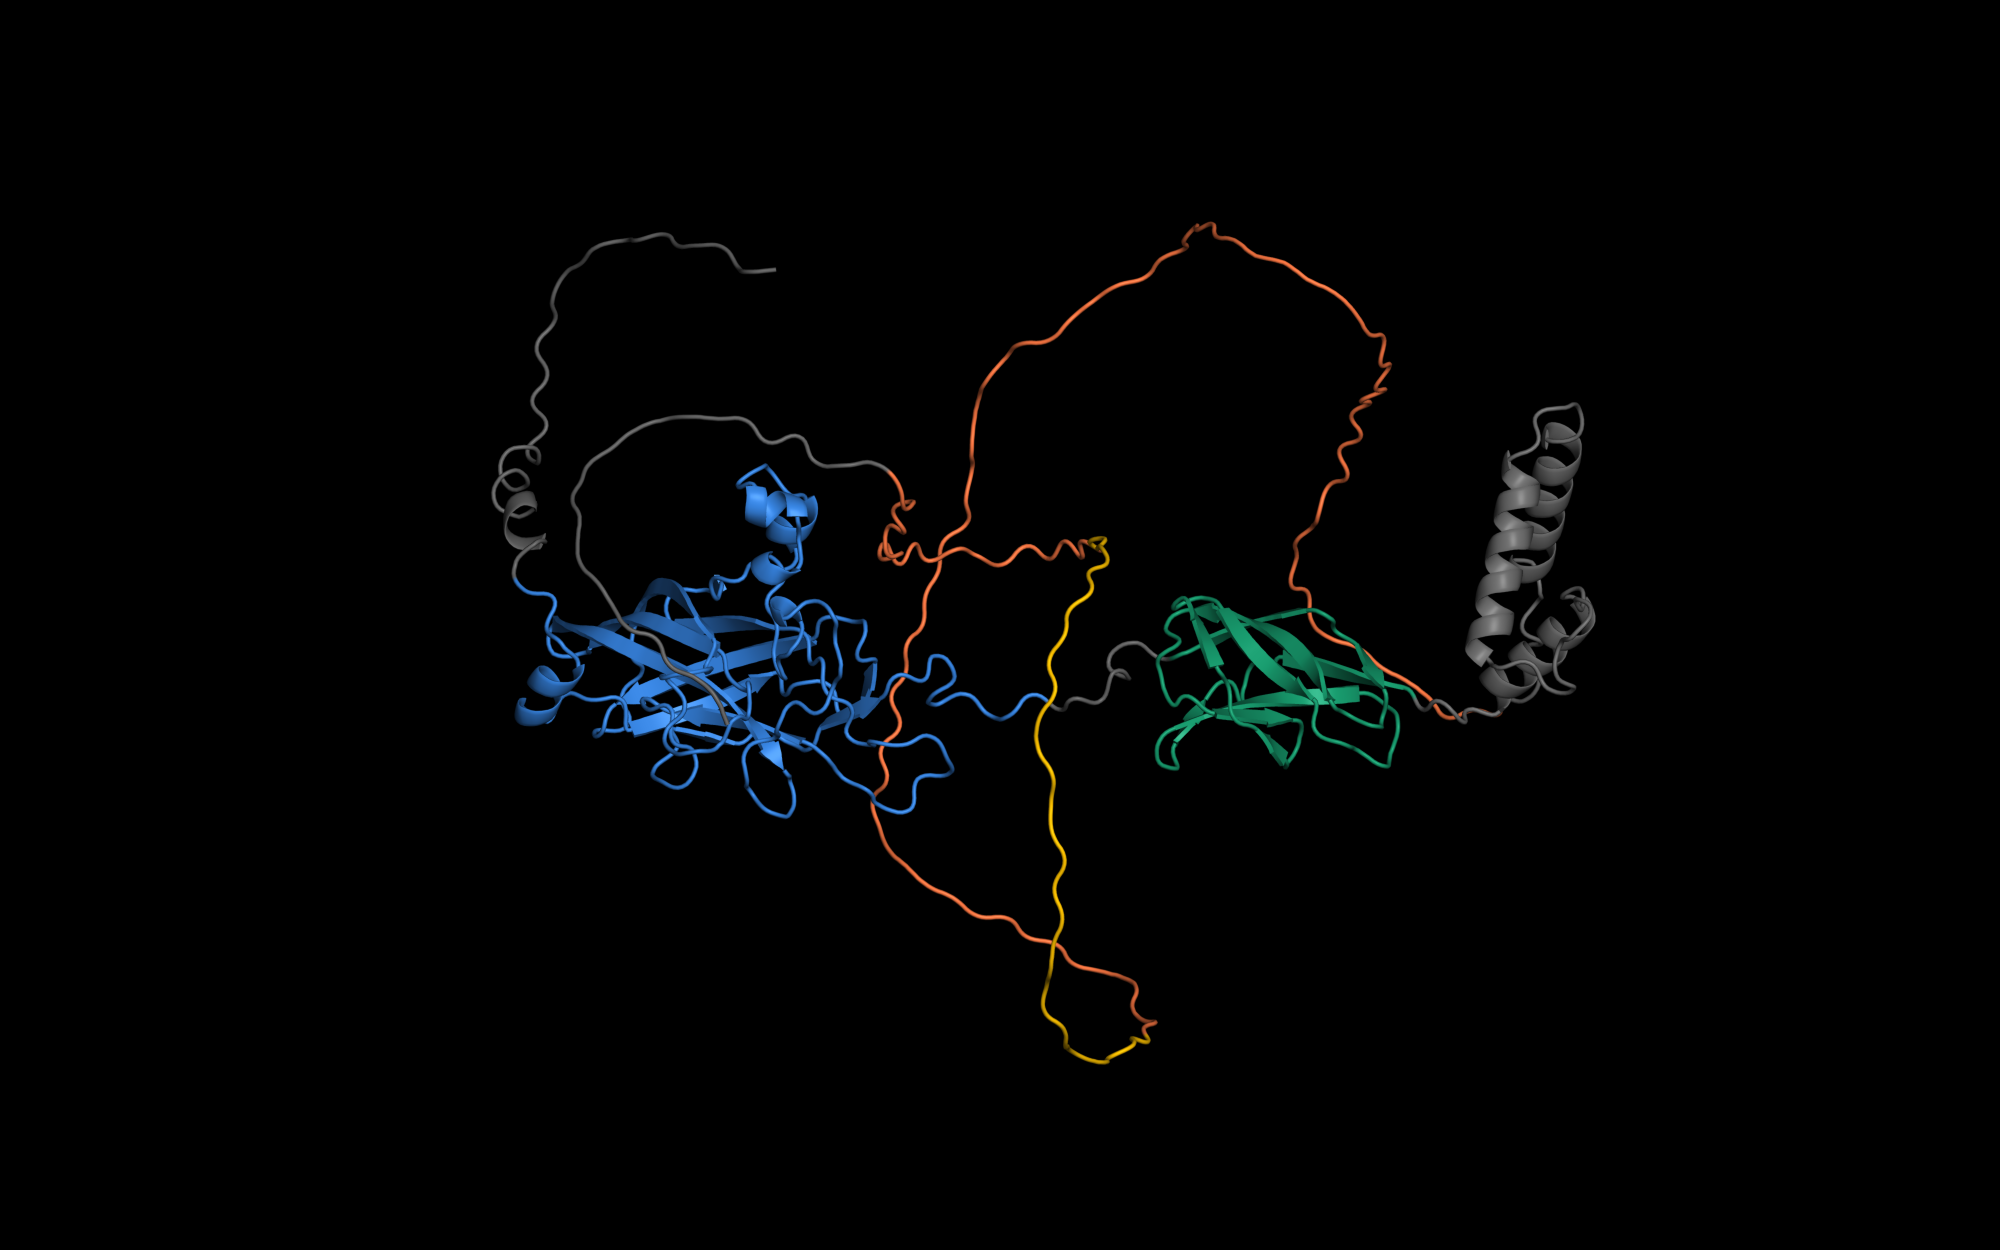
\includegraphics[width=0.95\textwidth]{figures/raport_ebf2_epitop.png}
\caption{Model AlphaFold białka EBF2 myszy. Kolor niebieski, domena wiążąca DNA
(reszty 34 do 244). Zielony, domena IPT/TIG (253 do 336). Szary w środku,
trzy helisy odpowiadające za łączenie się białek w pary (337 do 412).
\textbf{Pomarańczowy, fragment rozpoznawany przez przeciwciało} (413 do 550),
kolor żółty to jego rdzeń (496 do 528). Rycina wykonana skryptem
\texttt{45\_fig\_epitop\_czarne.pml}.}
\end{figure}

\section{Dlaczego akurat ten fragment białka}

W komórkach Purkinjego jest też białko pokrewne, EBF1. Jest go \textbf{sześć i pół
raza więcej} niż EBF2 (20,5 kontra 3,1 CP10K) i jest obecne w 99,9 procentach jąder,
przy czym \textbf{nie różnicuje} grup Aldoc. Przeciwciało, które myliłoby oba białka,
zniosłoby cały rozdział.

Porównanie sekwencji obu białek pokazuje, gdzie da się je odróżnić:

\begin{table}[h]
\centering
\begin{tabular}{lr}
\toprule
Obszar białka & Podobieństwo EBF2 do EBF1 \\
\midrule
Domena wiążąca DNA & 95,5 \% \\
Domena IPT/TIG & 96,4 \% \\
\textbf{Koniec C (413 do 550)} & \textbf{62,2 \%} \\
\bottomrule
\end{tabular}
\caption{Odróżnić je można tylko na końcu C. Skrypt \texttt{39\_ebf2\_struktura\_fig.py}.}
\end{table}

Przeciwciało \texttt{HPA003954} rozpoznaje fragment 412 do 550, czyli dokładnie ten
obszar. Sprawdzono dopasowanie tego fragmentu do białek myszy:
\textbf{100 procent zgodności z mysim EBF2} (138 na 138 reszt), 60,3 procent z EBF1
i 71,8 procent z EBF3.

Ten fragment nie ma własnej struktury przestrzennej. Spośród 138 reszt
\textbf{żadna} nie osiąga progu wiarygodności modelu. To dobrze dla przeciwciała:
fragment sterczy na zewnątrz i jest dostępny bez dodatkowej obróbki próbki.

\section{Czego można się spodziewać na cytometrze}

\begin{figure}[h]
\centering
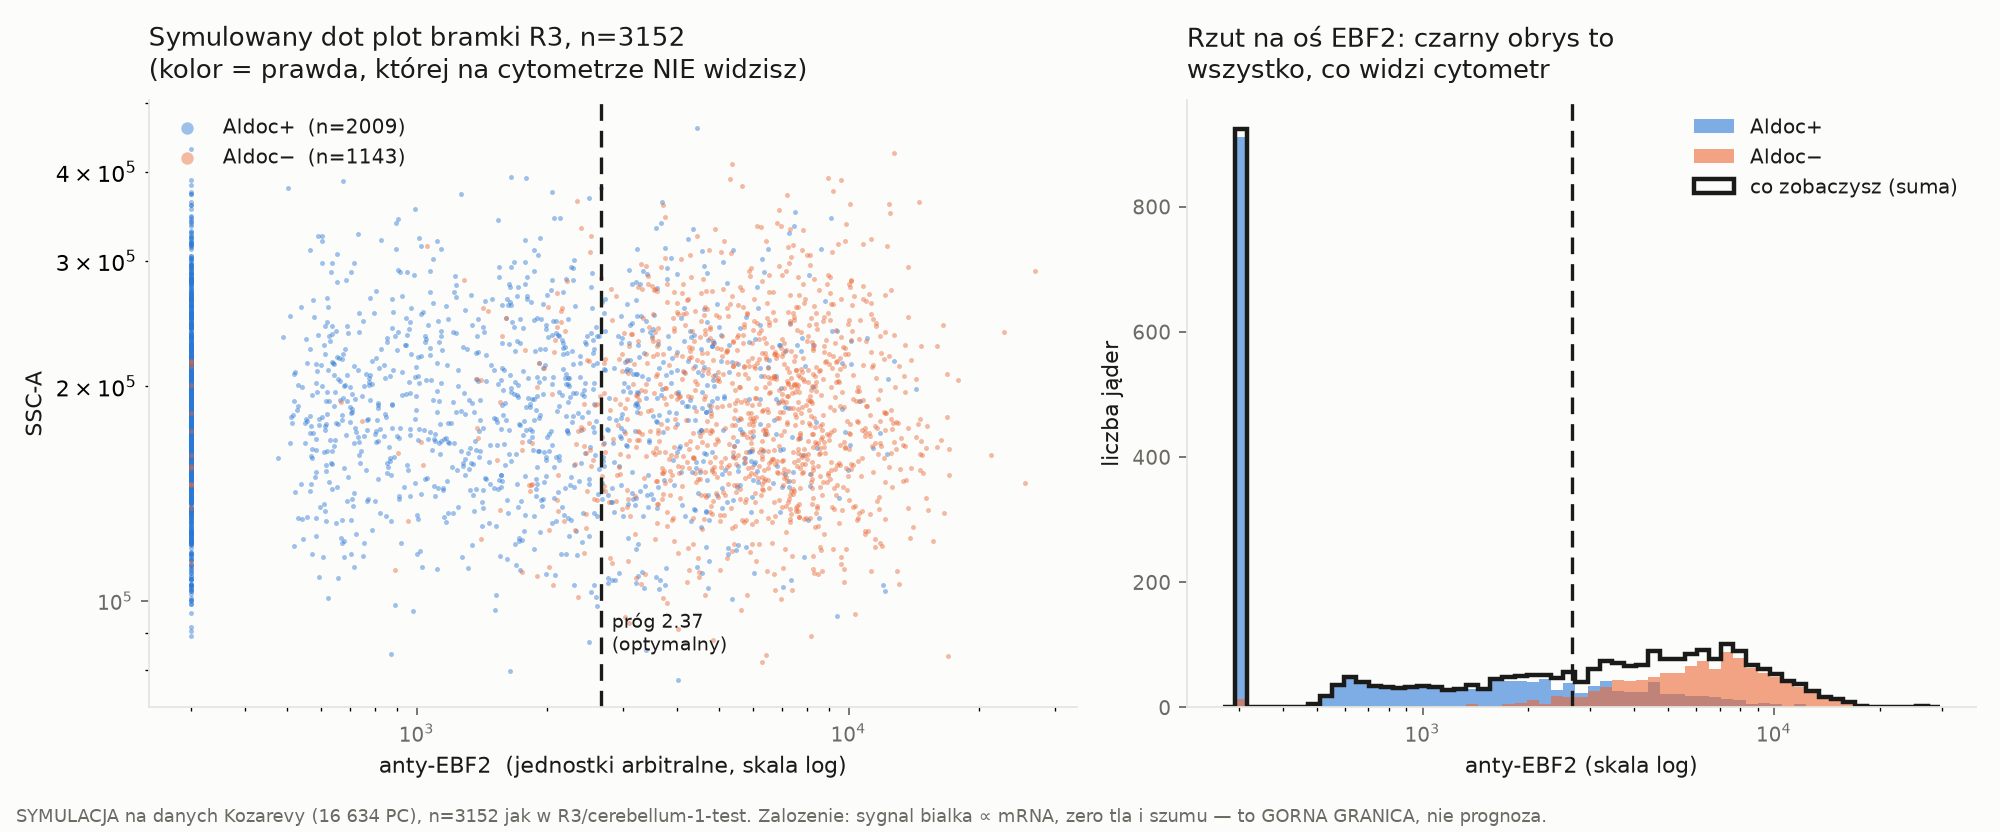
\includegraphics[width=\textwidth]{figures/symulacja_bramka_ebf2.png}
\caption{Symulacja wykresu punktowego dla bramki R3 przy 3 152 zdarzeniach,
czyli tylu, ile było w próbce cerebellum-1-test. Kolory pokazują prawdę, której
na cytometrze nie widać. Czarny obrys po prawej to wszystko, co widzi aparat.
Skrypt \texttt{43\_symulacja\_bramki\_ebf2.py}.}
\end{figure}

Wniosek jest taki: \textbf{nie zobaczy się dwóch osobnych skupisk}. Będzie jedno
skupisko rozciągnięte wzdłuż osi sygnału, z zagęszczeniem przy dolnej krawędzi.
Granicę bramki trzeba będzie ustawić umownie, a nie w naturalnym przewężeniu.

Przy najlepszym możliwym progu czystość wyniesie:

\begin{table}[h]
\centering
\begin{tabular}{lrr}
\toprule
Bramka & Liczba jąder & Czystość \\
\midrule
Sygnał niski, czyli Aldoc dodatnie & 1 724 & \textbf{94,5 \%} \\
Sygnał wysoki, czyli Aldoc ujemne & 1 428 & 73,5 \% \\
\bottomrule
\end{tabular}
\caption{Symulacja przy 3 152 zdarzeniach.}
\end{table}

\section{Trzy powody, dla których w rzeczywistości będzie gorzej}

\begin{enumerate}
    \item Te 47 procent jąder Aldoc dodatnich bez odczytu to w dużej części
    ograniczenie metody snRNA-seq, a nie faktyczny brak białka. Zera sztucznie
    rozsuwają obie grupy.
    \item Białko utrzymuje się w komórce dłużej niż mRNA, więc uśrednia różnice.
    \item Przeciwciało daje tło, którego w danych o mRNA nie ma wcale.
\end{enumerate}

Wartość 0,932 należy więc traktować jako \textbf{górną granicę}, a nie jako
przewidywany wynik.

\chapter{Podsumowanie}

\begin{itemize}
    \item Twierdzenie pierwsze jest \textbf{potwierdzone} i przeszło cztery próby
    obalenia. Różnica w poziomie mRNA \textit{Ebf2} między grupami jest duża
    i nie wynika z próbki, położenia w móżdżku, głębokości odczytu ani błędu w kodzie.

    \item Twierdzenie drugie to \textbf{przewidywanie}. Kierunek przesunięcia
    jest niemal pewny, ale rozdział będzie stopniowy, a nie dwuskupiskowy.

    \item \textbf{Nikt dotąd nie zmierzył białka EBF2 w tych komórkach cytometrycznie.}
    Żadne z dostępnych przeciwciał nie ma potwierdzenia do cytometrii przepływowej.

    \item Do pierwszego podejścia warto wziąć przeciwciało \texttt{AF7006} bez
    barwnika wraz z przeciwciałem drugorzędowym, ponieważ daje ono wzmocnienie
    sygnału. Jest owcze, więc nie koliduje z mysim przeciwciałem przeciw RanBP2
    zajmującym kanał 488.

    \item Konieczna jest kontrola bez przeciwciała przeciw EBF2. Bez niej,
    wobec braku naturalnego przewężenia, granica bramki byłaby dowolna.
\end{itemize}

\end{document}
